\documentclass[tikz,border=10pt]{standalone}
% Scale s = 0.015385 cm per pixel (longest ink side = 8 cm)
\begin{document}
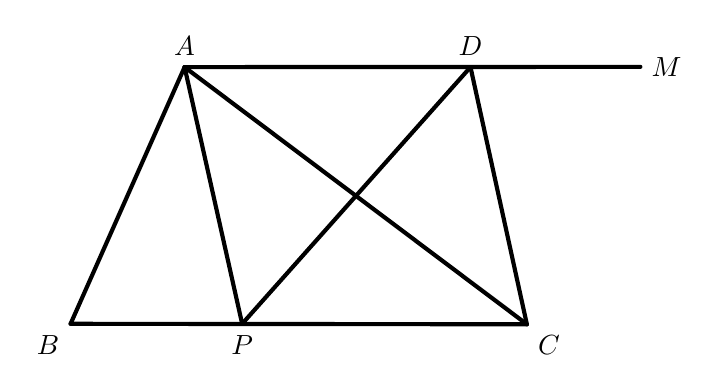
\begin{tikzpicture}[line width=1.5pt, line join=round, line cap=round]
  % Named points (coordinates unchanged from v1)
  \coordinate (B) at (-3.514,-1.623);
  \coordinate (P) at (-1.335,-1.623);
  \coordinate (C) at (2.281,-1.629);
  \coordinate (A) at (-2.066,1.637);
  \coordinate (D) at (1.565,1.637);
  \coordinate (M) at (3.723,1.640);

  % Bottom line B--C (through P)
  \draw (B) -- (C);
  % Top line A--M (through D)
  \draw (A) -- (M);
  % Remaining segments
  \draw (B) -- (A);
  \draw (A) -- (P);
  \draw (A) -- (C);
  \draw (P) -- (D);
  \draw (D) -- (C);

  % Labels, placed after all draw commands
  \node[above] at (A) {$A$};
  \node[above] at (D) {$D$};
  \node[right] at (M) {$M$};
  \node[below left] at (B) {$B$};
  \node[below] at (P) {$P$};
  \node[below right] at (C) {$C$};
\end{tikzpicture}
\end{document}